\documentclass[a4paper]{article}

\usepackage[russian]{babel}
\usepackage[left=1cm, right=1cm, top=1cm, bottom=1cm]{geometry}

\usepackage{graphicx}
\usepackage{multicol}
\usepackage{amssymb}
\usepackage{amsmath}
%\usepackage{multline}

\newcommand{\solutionstart}{{\noindent $\square$ \\}}
\newcommand{\solutionend}{{\noindent $\blacksquare$ \\}}

\begin{document}

\pagestyle{empty}

\section{Задания}

\begin{multicols}{2}

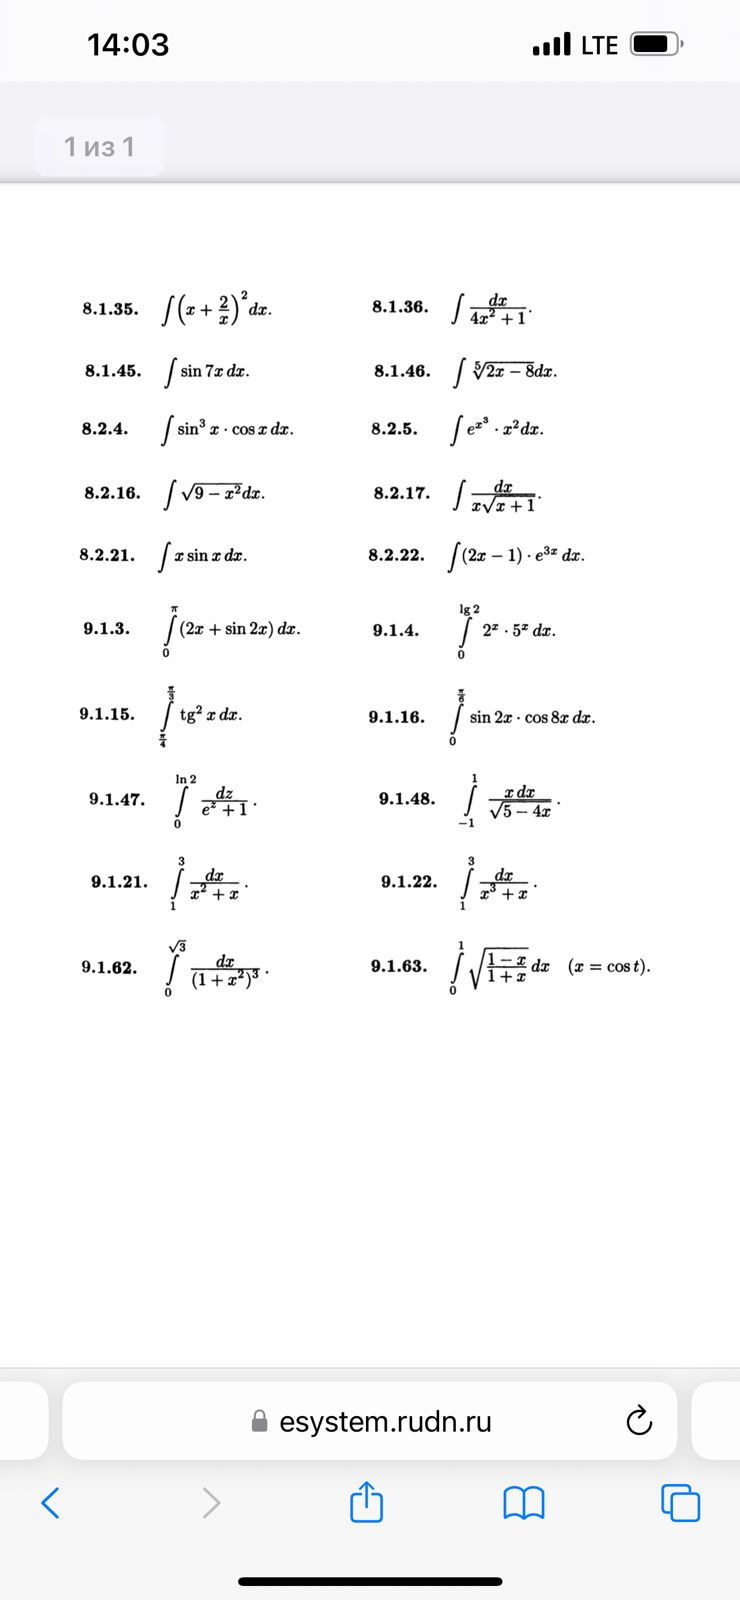
\includegraphics[width=8cm]{photo_1.jpg}


\includegraphics[width=8cm]{photo_2.jpg}

\end{multicols}



\section{Решения}

\subsection{}
Исследуйте на устойчивость нулевое решение уравнения:
\[
	f(t + 2) - 2 f (t + 1) + 5 f(t) = 0.
\]

\solutionstart
Указанное выражение является линейным однородным разностным уравнением 2-го порядка с постоянными коэффициентами. В общем случае такого уравнения для $n$ порядка:
\[
a_0 f (t + n) + a_1 f(t + n - 1) + ... + a_{n-1} f(t + 1) + a_n f(t) = 0
\]
единственное стационарное решение является нулевым. Для 
\begin{enumerate}
\item \textbf{устойчивости} такого решения необходимо и достаточно, чтобы модуль каждого из решений характеристического уравнения $P(\lambda) = a_{0} \lambda^{n} + a_{1} \lambda^{n - 1} + ... + a_{n - 1} \lambda + a_{n} = 0$ был меньше либо равен единице $|\lambda_j| \le 1$ и корни, по модулю равные единице, являлись простыми числами (единичной кратности).
\item \textbf{асимптотической устойчивости} такого решения необходимо и достаточно, чтобы модуль каждого из решений характеристического уравнения был меньше единицы $|\lambda_j| < 1$.
\end{enumerate}

\textbf{Теорема Шура:} Корни характеристического уравнения по модулю меньше единицы тогда и только тогда, когда специальные определители, сформированные из коэффициентов этого уравнения, положительны $\Delta_j|_{j=1..n} > 0$:

\[
\Delta_1 = 
\begin{vmatrix}
a_0 & a_n \\
a_n & a_0
\end{vmatrix},
\]

\[
\Delta_2 = 
\begin{vmatrix}
a_0 & 0 & a_n & a_{n - 1} \\
a_1 & a_0 & 0 &  a_n \\
a_n & 0 & a_0 & a_1 \\
a_{n-1} & a_n & 0 & a_0
\end{vmatrix},
\]
\[ \dots \]
\[
\Delta_n = 
\begin{vmatrix}
a_0 & 0 & \dots & 0 & a_n & a_{n-1} & \dots & a_1 \\
a_1 & a_0 &  & 0 & 0 & a_n &  & a_2 \\
\vdots &  & \ddots & & \vdots &  & \ddots & \\
a_{n-1} &  &  & a_0 & 0 & 0 & 0 & a_{n} \\
a_{n} & 0 & \dots & 0 & a_0 & a_1 & \dots & a_{n-1} \\
a_{n-1} & a_n & &  & 0 & a_0 &  & a_{n-2} \\
\vdots &  & \ddots &  & \vdots &  & \ddots &  \\
a_1 &  &  & a_n & 0 & 0 & 0 & a_0 \\
\end{vmatrix}.
\]

В дальнейшем будем находить корни характеристического уравнения напрямую и для сравнения вычислять указанные выше определители. В силу эквивалентности такие проверки должны давать одинаковый результат.

Составим характеристическое уравнение для рассматриваемого случая:
\[
\lambda^2 - 2 \lambda + 5 = 0.
\]
Его корни: $\lambda_1 = 1 - 2i$, $\lambda_2 = 1 + 2i$, модули корней: $\lambda_1 = \lambda_2 \simeq 2.23$. Определители: $\Delta_1 = -24$, $\Delta_2 = 512$. Видно, что модули корней характеристического уравнений больше единицы, один из определителей меньше нуля, а значит нулевое решение \textit{не является устойчивым}.

\solutionend

\subsection{}
Исследуйте на устойчивость нулевое решение уравнения:
\[
	f(t + 4) + f (t + 3) + f(t) = 0.
\]

\solutionstart
Характеристическое уравнение: 
\[
\lambda^4 + \lambda^3 + 1 = 0.
\]
Полная запись корней уравнения является громоздкой, поэтому приведем сразу модули корней: $\lambda_1 = \lambda_2 \simeq 1.18$, $\lambda_3 = \lambda_4 \simeq 0.84$. Определители: $\Delta_1 = 0$, $\Delta_2 = -1$, $\Delta_3 = -1$, $\Delta_4 = 3$. Видно, что два корня характеристического уравнения по модулю больше единицы, два определителя меньше нуля, значит нулевое решение \textit{не является устойчивым}.

\solutionend


\subsection{}
Исследуйте на устойчивость нулевое решение уравнения:
\[
	7 f(t + 4) - 4 f (t + 3) + 30 f(t + 2) - 4 f(t + 1) + 3 f(t) = 0.
\]

\solutionstart
Характеристическое уравнение: 
\[
7 \lambda^4 - 4 \lambda^3 + 30 \lambda^2 - 4 \lambda + 3 = 0.
\]

Полная запись корней уравнения является громоздкой, поэтому приведем сразу модули корней: $\lambda_1 = \lambda_2 \simeq 0.32$, $\lambda_3 = \lambda_4 \simeq 2.03$. Определители: $\Delta_1 = 40$, $\Delta_2 = 1344$, $\Delta_3 = -471040$, $\Delta_4 = 157286400$. Видно, что два корня характеристического уравнения по модулю больше единицы, $\Delta_3$ меньше нуля, значит нулевое решение \textit{не является устойчивым}.

\solutionend


\subsection{}
Найдите необходимое и достаточное условие асимптотической устойчивости нулевого решения разностного уравнения:
\[
	a_0 f (t + 3) + a_1 f(t + 2) + a_2 f(t + 1) + a_3 f(t) = 0.
\]

\solutionstart

Характеристическое уравнение:
\[
	a_0 \lambda^3 + a_1 \lambda^2 + a_2 \lambda + a_3 = 0.
\]

Полная запись корней характеристического уравнения является громоздкой, поэтому запишем необходимое и достаточное условие асимптотической устойчивости через определители:
\[
\Delta_1 = a_0^2 - a_3^2 > 0,
\]
\[
\Delta_2 = a_0^4 - a_0^2 a_2^2 - 2 a_0^2 a_3^2 + 2 a_0 a_1 a_2 a_3 - a_1^2 a_3^2 + a_3^4 > 0,
\]
\begin{gather*}
\Delta_3 = a_0^6 - a_0^4 a_1^2 - 2 a_0^4 a_2^2 - 3 a_0^4 a_3^2 + 2 a_0^3 a_1^2 a_2 + 6 a_0^3 a_1 a_2 a_3 - 2 a_0^2 a_1^3 a_3 - a_0^2 a_1^2 a_2^2 - a_0^2 a_1^2 a_3^2 -\\- 4 a_0^2 a_1 a_2^2 a_3 + a_0^2 a_2^4 + a_0^2 a_2^2 a_3^2 + 3 a_0^2 a_3^4 + 2 a_0 a_1^3 a_2 a_3 + 4 a_0 a_1^2 a_2 a_3^2 - 2 a_0 a_1 a_2^3 a_3 - 6 a_0 a_1 a_2 a_3^3 + 2 a_0 a_2^3 a_3^2 - a_1^4 a_3^2 +\\+ a_1^2 a_2^2 a_3^2 + 2 a_1^2 a_3^4 - 2 a_1 a_2^2 a_3^3 + a_2^2 a_3^4 - a_3^6 > 0.
\end{gather*}

\solutionend


\subsection{}
Найдите необходимое и достаточное условие асимптотической устойчивости нулевого решения разностного уравнения:
\[
	f (t + 4) + p f(t + 3) + q f(t) = 0.
\]

\solutionstart

Характеристическое уравнение:
\[
	\lambda^4 + p \lambda^3 + q = 0.
\]

Полная запись корней характеристического уравнения является громоздкой, поэтому запишем необходимое и достаточное условие асимптотической устойчивости через определители:
\[
\Delta_1 = 1 - q^2 > 0,
\]
\[
\Delta_2 = -p^2 q^2 + q^4 - 2 q^2 + 1 > 0,
\]
\[
\Delta_3 = -p^4 q^2 + 2 p^2 q^4 - 2 p^2 q^2 - q^6 + 3 q^4 - 3 q^2 + 1 > 0,
\]
\[
\Delta_4 = -p^6 q^2 + 3 p^4 q^4 - p^4 q^2 + 2 p^4 q - 3 p^2 q^6 + 5 p^2 q^4 - p^2 q^2 - p^2 + q^8 - 4 q^6 + 6 q^4 - 4 q^2 + 1 > 0.
\]

\solutionend


\subsection{}
Найдите необходимое и достаточное условие асимптотической устойчивости нулевого решения разностного уравнения:
\[
	f (t + 5) + p f(t) = 0.
\]

\solutionstart

Характеристическое уравнение:
\[
	\lambda^5 + p \lambda = 0.
\]

Полная запись корней характеристического уравнения является громоздкой, поэтому запишем необходимое и достаточное условие асимптотической устойчивости через определители:
\[
\Delta_1 = 1 - p^2 > 0,
\]
\[
\Delta_2 = (1 - p^2)^2 > 0,
\]
\[
\Delta_3 = (1 - p^2)^3 > 0,
\]
\[
\Delta_4 = (1 - p^2)^4 > 0,
\]
\[
\Delta_5 = (1 - p^2)^5 > 0.
\]

Исходя из представленных выражений для определителей, решение уравнения будет асимптотически устойчиво при $p < 1$.


\subsection{}
Пусть динамика численности популяции описывается дискретным уравнением:
\[
N_{t + 1} = a N_t - N_t, (a > 1)
\]
Найдите положения равновесия. Исследуйте характер каждого из найденных положений равновесия в зависимости от параметра $a$.

\solutionstart
В случае тривиального начального условия $N_0 = 0$ система с первого шага войдет в положение устойчивого равновесия, соответствующее нулевым значениям $N_t$ вне зависимости от параметра $a$. При $N_0 = 1$ cистема также устойчива вне зависимости от $a$, поскольку на каждом следующем шаге $N_{t + 1} = a - 1$. Аналогичный результат наблюдается при любом значении $a$, если $N_0 = a - 1$. При возрастании $N_0$ устойчивость системы будет зависеть от соотношения между линейной составляющей с коэффициентом $a$ и квадратичным слагаемым. В некоторых случаях достигается равновесие: \{$a = 2.5$, $N_0 = 1.7$\}, \{$a = 2.8$, $N_0 = 2.0$\}, в некоторых -- хаос: \{$a = 3.8$, $N_0 = 1.1$\}, \{$a = 4.0$, $N_0 = 0.9$\}.

\solutionend



\subsection{}
Пусть динамика численности популяции описывается дискретным уравнением:
\[
N_{t + 1} = a N_t - N_t, (a > 1)
\]
Постройте лестницу Ламерея и определите значения $N_1$, $N_2$, $N_3$, $N_4$, $N_5$, если $a = 2.5$ и $N_0 = 1.7$. Постройте соответствующую временную динамику $N(t)$.

\solutionstart

Решим указанное уравнение для заданных параметров и получим: $N_1 \simeq 1.36$, $N_2 \simeq 1.55$, $N_3 \simeq 1.47$, $N_4 \simeq 1.51$, $N_5 \simeq 1.49$. Временная динамика и лестница Ламерея представлены на рисунках ниже. В лестнице Ламерея для ясности восприятия приведены только несколько первых итераций.

\begin{tabular}{p{8cm}p{8cm}}
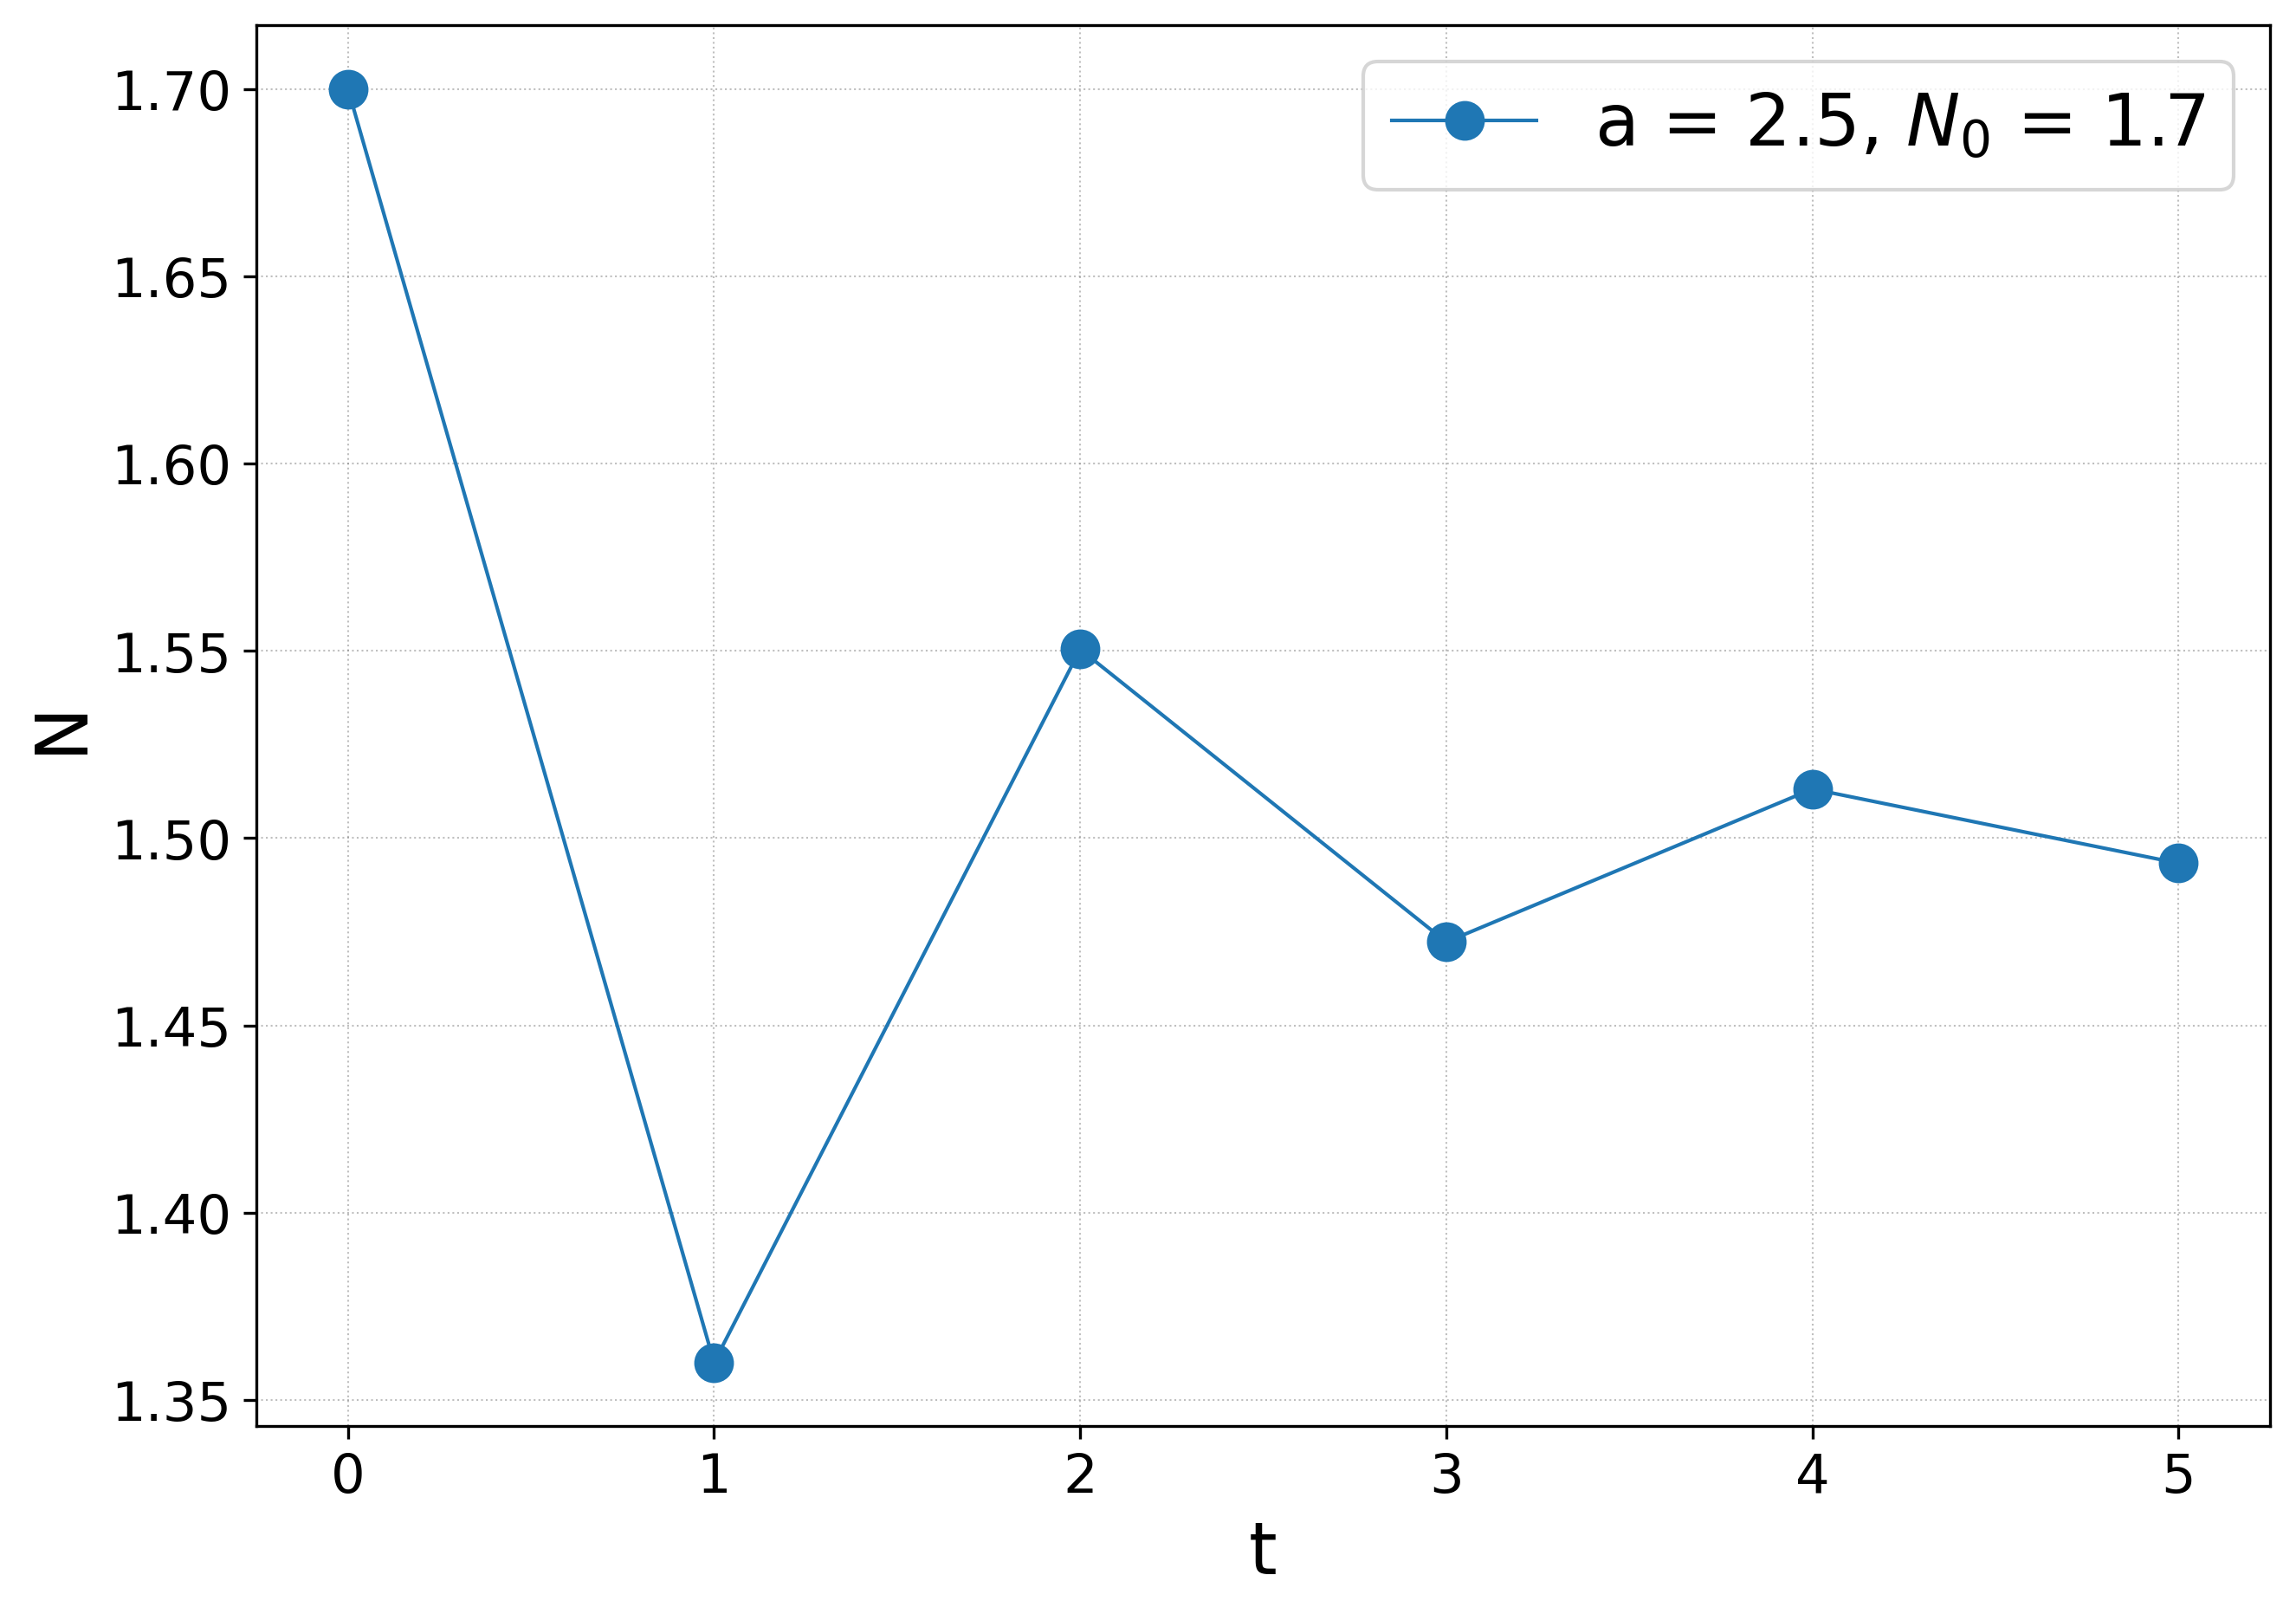
\includegraphics[width=\linewidth]{N(t).png} &
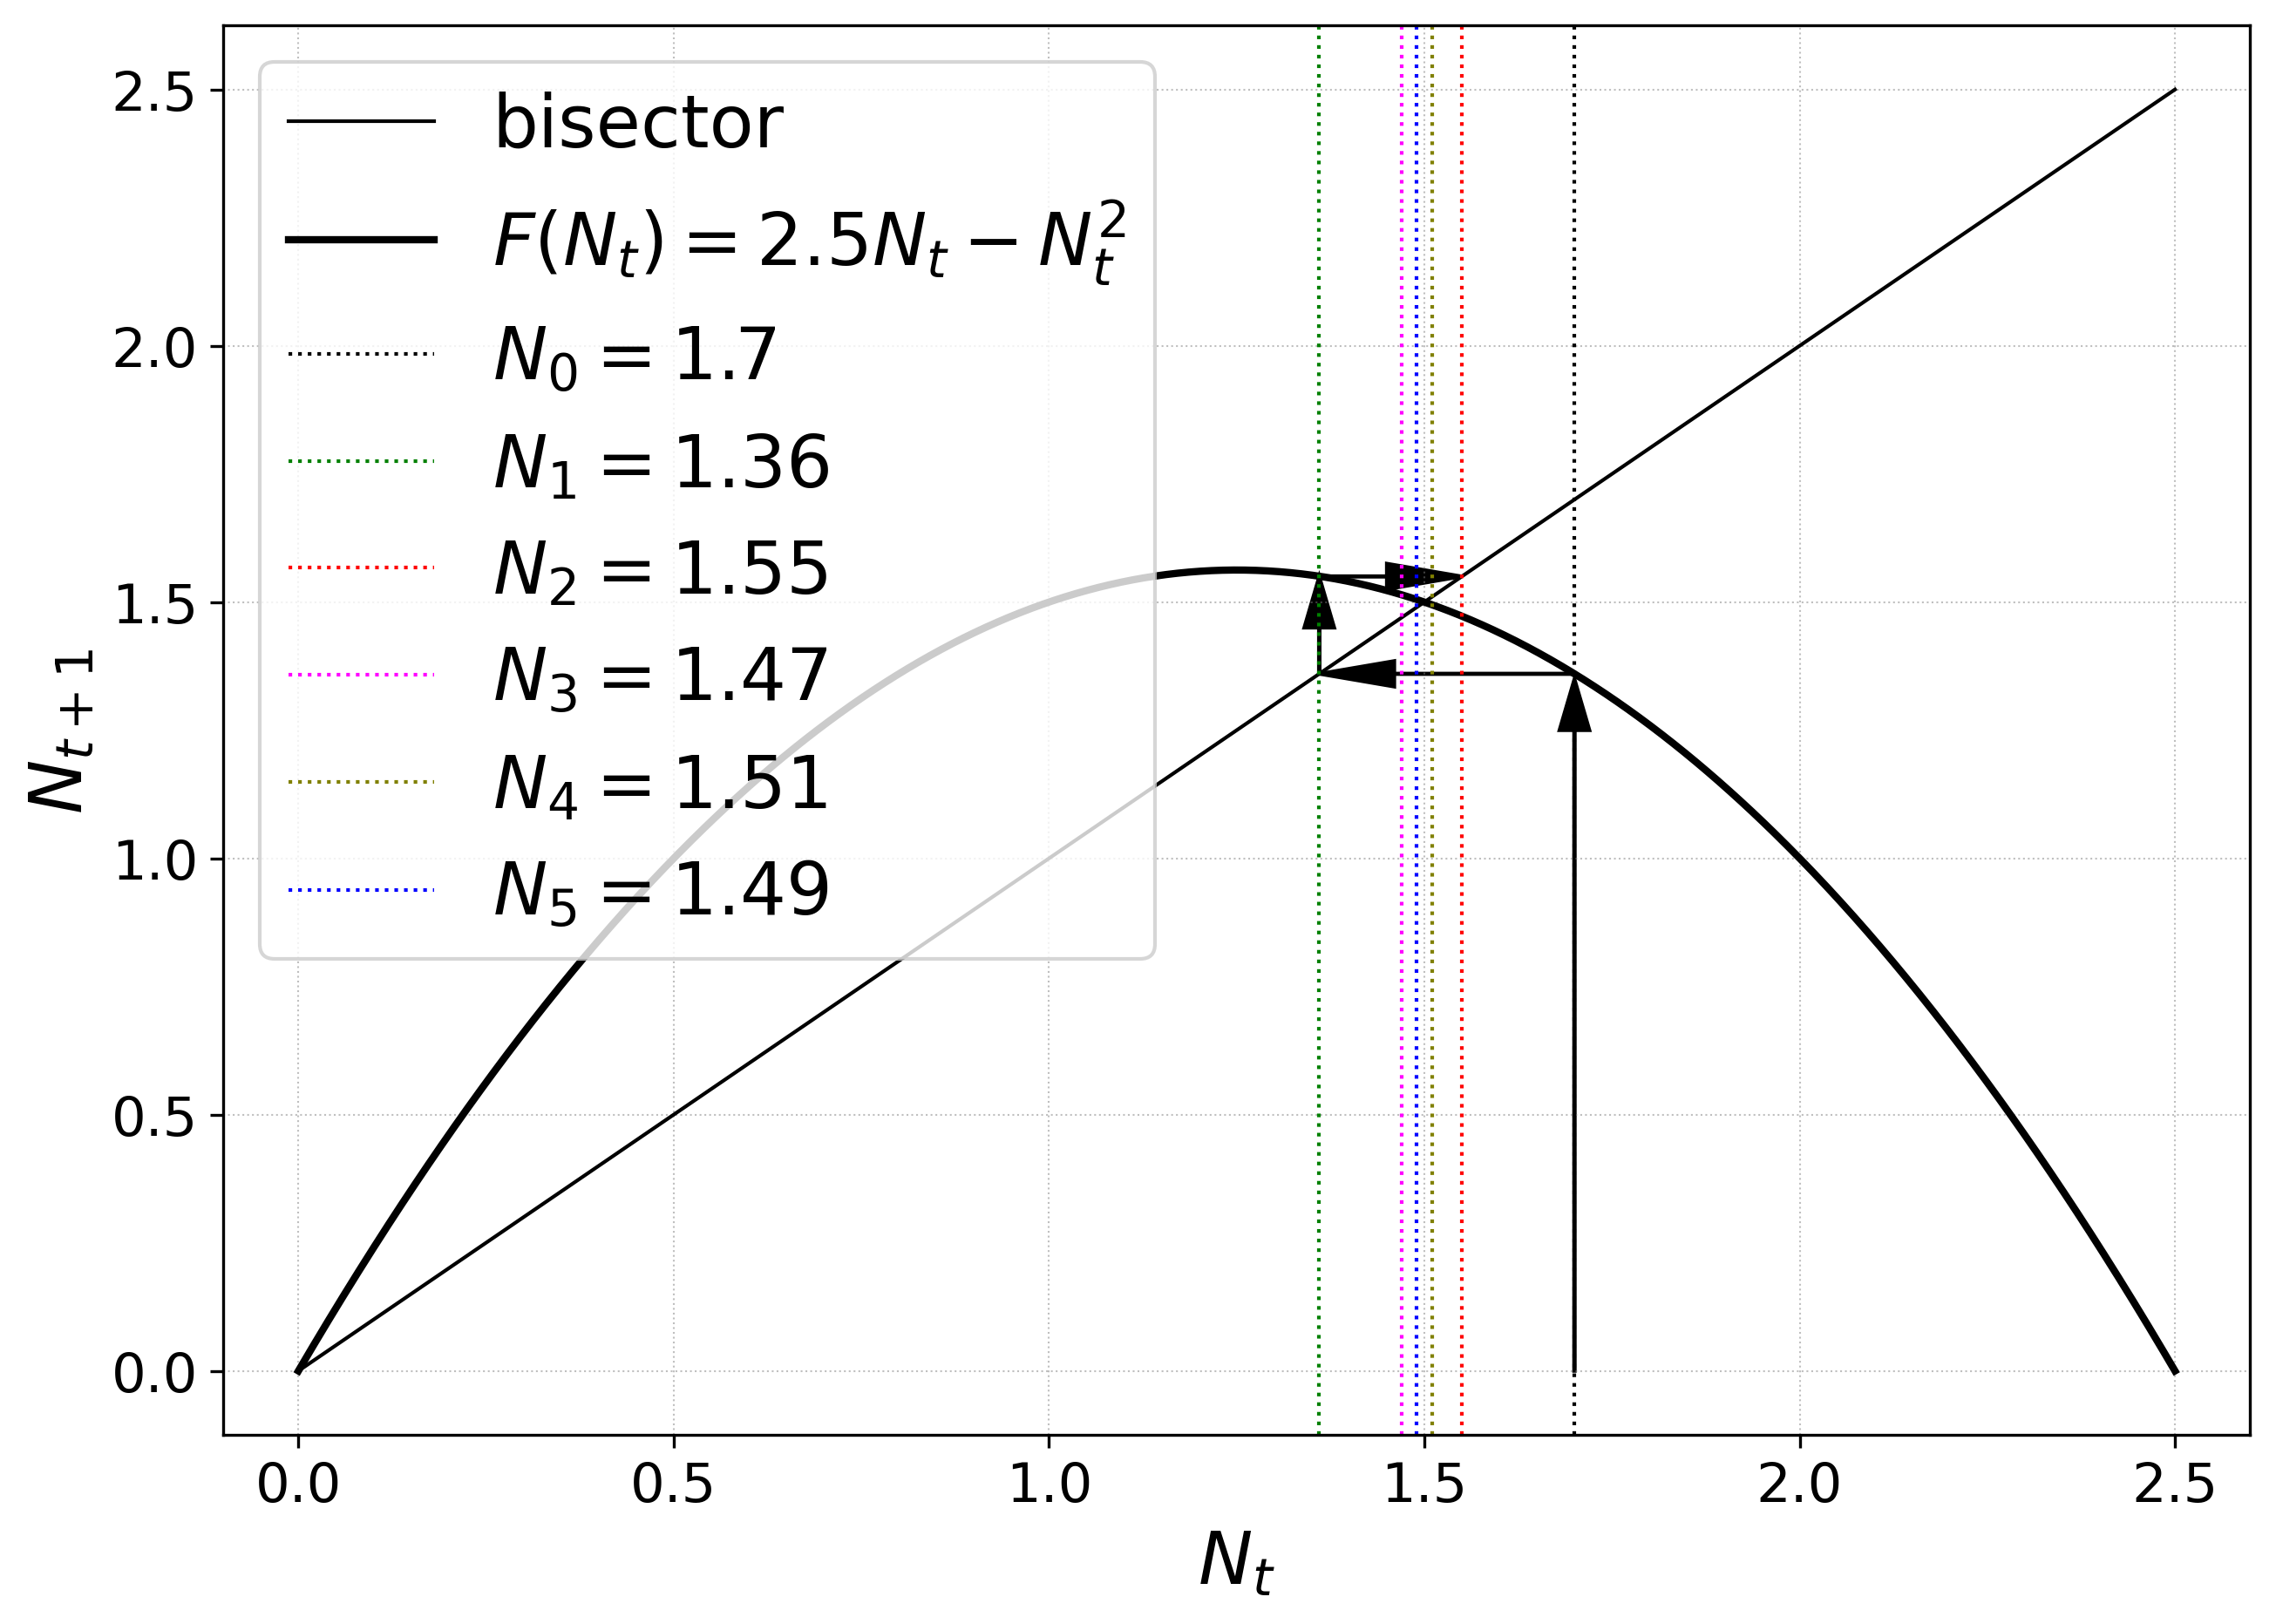
\includegraphics[width=\linewidth]{stairs.png} \\
\centering{Временная динамика} & \centering{Лестница Ламерея}
\end{tabular}

\solutionend

\subsection{}
Пусть динамика численности популяции описывается дискретным уравнением:
\[
N_{t + 1} = a N_t - N_t, (a > 1)
\]
Укажите характер ненулевой неподвижной точки (устойчивая, неустойчивая) и тип динамического поведения модели вблизи этой точки (монотонный рост, колебания, хаотический режим).


\solutionstart
В приблизительно в районе точки $N \simeq 1.5$ наблюдается устойчивое равновесие с колебательным поведением модели.

\solutionend

\end{document}